% Layout uses only packages present in the local TinyTeX install:
% psnfss (mathptmx, helvet), geometry, amsmath/amssymb, xcolor, booktabs,
% tools (array, tabularx), natbib, hyperref.
\documentclass[11pt,letterpaper]{article}
\usepackage[T1]{fontenc}
\usepackage[utf8]{inputenc}
\usepackage{amsmath,amssymb}
\usepackage{mathptmx}
\DeclareSymbolFont{symbols}{OMS}{cmsy}{m}{n}
\DeclareMathAlphabet{\mathcal}{OMS}{cmsy}{m}{n}
\usepackage[scaled=0.90]{helvet}
\usepackage[margin=0.9in,headsep=12pt,footskip=24pt]{geometry}
\usepackage{xcolor}
\usepackage{booktabs,array,tabularx}
\usepackage{graphicx}
\usepackage[numbers,sort&compress]{natbib}
\usepackage[colorlinks=true,linkcolor=navy,citecolor=navy,urlcolor=navy]{hyperref}
\urlstyle{same}

% ---------------------------------------------------------------- colours
\definecolor{navy}{HTML}{1F3A5F}
\definecolor{slate}{HTML}{5B6770}
\definecolor{tint}{HTML}{E9EEF4}
\definecolor{rulegray}{HTML}{B8C2CC}

% ---------------------------------------------------------------- spacing
\setlength{\parindent}{0pt}
\setlength{\parskip}{0.45em}
\linespread{1.02}
\setlength{\intextsep}{10pt}
\setlength{\textfloatsep}{12pt}
\setlength{\abovecaptionskip}{4pt}
\setlength{\belowcaptionskip}{4pt}

\makeatletter
% Keep headings with their first lines (needspace logic; package not in TinyTeX).
\newcommand{\needspace}[1]{\par\penalty-100\begingroup\setlength{\dimen@}{#1}%
  \dimen@ii\pagegoal\advance\dimen@ii-\pagetotal
  \ifdim\dimen@>\dimen@ii\ifdim\dimen@ii>\z@\vfil\fi\break\fi\endgroup}
% Section headings: sans serif, black, numbered.
\renewcommand{\section}{\needspace{7\baselineskip}\@startsection{section}{1}{0pt}%
  {-2.0ex plus -.4ex minus -.2ex}{0.8ex plus .2ex}%
  {\sffamily\Large\bfseries\color{black}}}
\renewcommand{\subsection}{\needspace{5\baselineskip}\@startsection{subsection}{2}{0pt}%
  {-1.6ex plus -.3ex minus -.2ex}{0.5ex plus .1ex}%
  {\sffamily\normalsize\bfseries\color{black}}}

% Captions: "Table 1  Title" in sans; tables captioned above, figures below.
\long\def\@makecaption#1#2{%
  \vskip\abovecaptionskip
  {\sffamily\small{\bfseries\color{black}#1}\enspace #2\par}%
  \vskip\belowcaptionskip}
\renewcommand{\fnum@table}{Table~\thetable}
\renewcommand{\fnum@figure}{Figure~\thefigure}

% Running header and footer without extra packages.
\def\ps@report{%
  \def\@oddhead{\hfil{\sffamily\footnotesize\color{slate}Direct Indexing with Tax-Loss Harvesting}}%
  \let\@evenhead\@oddhead
  \def\@oddfoot{\hfil{\sffamily\footnotesize\color{slate}\thepage}\hfil}%
  \let\@evenfoot\@oddfoot}
\def\ps@firstpage{\let\@oddhead\@empty\let\@evenhead\@empty
  \def\@oddfoot{\hfil{\sffamily\footnotesize\color{slate}\thepage}\hfil}\let\@evenfoot\@oddfoot}
\makeatother
\pagestyle{report}

% Run-in finding headers inside subsections.
\newcommand{\lead}[1]{{\sffamily\bfseries\color{black}#1}\enspace}
% Compact lists without enumitem.
\newenvironment{tightitems}{\begin{list}{\textcolor{navy}{\small$\blacktriangleright$}}{%
  \setlength{\leftmargin}{1.3em}\setlength{\labelwidth}{1em}\setlength{\labelsep}{0.4em}%
  \setlength{\itemsep}{0.15em}\setlength{\parsep}{0pt}\setlength{\topsep}{0.2em}}}{\end{list}}

\renewcommand{\arraystretch}{1.18}
\newcolumntype{L}{>{\raggedright\arraybackslash}X}

\begin{document}
\thispagestyle{firstpage}
\setlength{\abovedisplayskip}{6pt}
\setlength{\belowdisplayskip}{6pt}
\setlength{\abovedisplayshortskip}{3pt}
\setlength{\belowdisplayshortskip}{4pt}

% ---------------------------------------------------------------- title block
\begingroup\sffamily
{\LARGE\bfseries Direct Indexing with Tax-Loss Harvesting\par}
\vspace{5pt}
{\large\color{slate}A Two-Step Tax- and Wash-Sale-Aware Optimization Strategy on the S\&P~500\par}
\vspace{10pt}
{\normalsize\bfseries Long Qian\par}
\vspace{1pt}
{\small\color{slate}November 2026\par}
\endgroup
\vspace{6pt}
{\color{black}\rule{\linewidth}{0.8pt}}
\vspace{4pt}

\section{Background}
\label{sec:background}

Direct indexing replicates a market index by holding its constituent stocks directly rather than through an ETF. This allows investors to manage individual positions and tax lots while maintaining broad market exposure.

A key advantage is tax-loss harvesting (TLH), which realizes losses on depreciated securities to offset taxable capital gains. Unlike index ETFs, direct indexing enables harvesting at the individual stock level. However, harvesting trades may introduce tracking error and transaction costs. Moreover, as portfolios age and unrealized gains accumulate, harvesting opportunities may decline, creating a trade-off between immediate tax benefits and long-term after-tax performance.

% Final strategy: outputs/ltfo_wash_a_det200_20261122_v3. Table 2 from results/decisions.jsonl.
\section{Methodology}
\label{sec:methodology}

The strategy holds S\&P~500 stocks directly and rebalances once a month. At each month-end close $t$, it sets target weights that minimize estimated tax plus trading cost while keeping ex-ante tracking error (TE) against the index below 1\%. 

Figure~\ref{fig:pipeline} shows the four stages. The optimizer reads current holdings, tax lots, and benchmark weights (Stage~1). It solves for target weights in two steps (Stage~2): first it decides whether to buy, sell or hold each stock with an unrealized loss, then it sizes all trades. Each sale relieves the lots with the lowest tax cost first (Stage~3), and orders execute at the next trading day's close (Stage~4). Sections~\ref{sec:data}--\ref{sec:tax} describe each part.

\begin{figure}[!h]
\centering
\newcommand{\stepbox}[2]{\fcolorbox{rulegray}{tint}{\parbox[t]{0.200\linewidth}{%
  \centering\sffamily{\tiny\bfseries\color{slate}#1\par}\vspace{2pt}
  \parbox[c][0.85cm][c]{\linewidth}{\centering\footnotesize\bfseries\color{black}#2}}}}
\newcommand{\steparrow}{\raisebox{-0.62cm}{\textcolor{navy}{$\boldsymbol{\rightarrow}$}}}
\setlength{\fboxsep}{5pt}%
\stepbox{STAGE 1 \,\textbar\, MONTH-END \textit{t}}{Weights / Tax Lots Input}%
\hfill\steparrow\hfill
\stepbox{STAGE 2 \,\textbar\, MONTH-END \textit{t}}{2-step Tax-aware Optimization}%
\hfill\steparrow\hfill
\stepbox{STAGE 3 \,\textbar\, MONTH-END \textit{t}}{Least-Tax-First-Out (LTFO)}%
\hfill\steparrow\hfill
\stepbox{STAGE 4 \,\textbar\, \textit{t}\,+\,1}{Execution}
\caption{Monthly rebalance process.}
\label{fig:pipeline}
\end{figure}

% ======================================================================
\subsection{Universe, Data and Timing}
\label{sec:data}

The backtest starts with \$1 million in cash in January 2016 and rebalances monthly through December 2025 (Table~\ref{tab:setup}). Because of non-accessibility to point-in-time S\&P~500 constituent weights, the universe and reference weights $b$ come from the month-end equity holdings of SPY, which fully replicates the index. Each month, targets are set with prices at the month-end close $t$ and traded at the next trading day's close $t{+}1$. Prices, total returns, dividends and corporate actions come from CRSP.

\begin{table}[!h]
\caption{Backtest specification}
\label{tab:setup}
\small
\begin{tabularx}{\linewidth}{@{}>{\leavevmode\sffamily\bfseries\color{black}}p{0.17\linewidth}L@{}}
\toprule
Time & Jan.~2016 -- Dec.~2025, 120 monthly rebalances \\
Initial Cash & \$1 million \\
Universe & Month-end SPY equity holdings (about 505 stocks), weights rescaled to 100\% \\
Benchmark & S\&P 500 Total Return Index \\
Timing & Optimize at month-end close, trade at the next trading day's close \\
Data & CRSP daily prices, total returns and corporate actions (WRDS) \\
Costs & 5 bp per side, no market impact, cash earns zero \\
Tax Rates & Short-term 40.8\%, long-term 23.8\%, dividends 23.8\% \\
Liquidation & No \\
Tax Settlement & Net annual tax paid from, or refunded to, the cash account on the first trading day of the next year, and refunds can be reinvested \\
\bottomrule
\end{tabularx}
\end{table}

Two simplifications introduce mild look-ahead: SPY's month-end holdings are assumed known at that day's close, and stocks about to be delisted are sold in advance using their known delisting date.

% ======================================================================
\subsection{Two-Step Tax-Aware Optimization}
\label{sec:optimization}

\lead{Objective.} Each month the two optimization steps choose target weights $w$ to minimize estimated tax benefits (differently defined in each step) plus trading cost, subject to long-only, fully invested and tracking-error constraints:
\begin{equation}
  \min_w\ J(w)=\frac{\gamma\,\mathrm{Tax}(w)+\mathrm{TC}(w)}{V}
  \qquad\text{s.t.}\quad w\ge0,\quad \mathbf 1^\top w=1,\quad \sqrt{(w-b)^\top\widehat\Sigma\,(w-b)}\le1\%,
  \label{eq:problem}
\end{equation}
where $V$ is portfolio value, $b$ the benchmark weights and $\widehat\Sigma$ a Ledoit--Wolf covariance from 252 daily returns. Stocks with shorter histories are held at benchmark weight. The transaction cost term is
\begin{equation}
  \widehat T(w)=\sum_\ell \tau_\ell\big[(1-c)P_{i(\ell)}-k_\ell\big]\,s_\ell(w),
  \qquad
  \mathrm{TC}(w)=c\sum_i\big|Vw_i-P_iq_i\big|,
  \label{eq:costs}
\end{equation}
where $s_\ell(w)$ is the number of shares sold from lot $\ell$, $k_\ell$ its per-share basis, $\tau_\ell$ the short- or long-term rate, $P_i$ the price, $q_i$ the shares held and $c=5$~bp. Lots with a loss contribute negative tax. Sales follow least-tax-first-out (LTFO): lots with the lowest tax per share are sold first. $\gamma$ is set to 0.5.

\lead{Why two steps.} For a stock holding a loss lot, estimated tax rises with $w_i$ up to the current weight and is flat above it. This kink makes \eqref{eq:problem} nonconvex. Fixing each such stock's trade direction removes the kink and leaves a convex problem (Moehle, Kochenderfer, Boyd and Ang, 2021).

\lead{Step 1: choose trade directions.} A local solver (SLSQP) searches \eqref{eq:problem} with tax adjusted for the 30-day wash-sale rule:
\begin{equation}
  \min_w\ J_1(w)=\frac{\gamma\big[\widehat T(w)+D_{\mathrm{sell}}(w)+D_{\mathrm{buy}}(w)\big]+\mathrm{TC}(w)}{V}
  \qquad\text{s.t. the constraints of \eqref{eq:problem}}.
  \label{eq:stage1}
\end{equation}
$D_{\mathrm{sell}}$ adds back the saving from a loss sale that matches shares bought in the past 30 days. $D_{\mathrm{buy}}$ adds back the saving from a past loss that a new purchase would disallow. Each stock with a loss lot is then labeled BUY, SELL or HOLD, and up to three distinct direction patterns are kept.

\lead{Step 2: size the trades.} For each direction pattern, the optimizer solves
\begin{equation}
\begin{aligned}
  \min_w\ \ & J_2(w)=\frac{\gamma\,\widehat T(w)+\mathrm{TC}(w)}{V}\\
  \text{s.t.}\ \ & \text{the constraints of \eqref{eq:problem}},\qquad
  w_i\ge h_i\ (\text{BUY}),\quad w_i\le h_i\ (\text{SELL}),\quad w_i=h_i\ (\text{HOLD}),
\end{aligned}
  \label{eq:stage2}
\end{equation}
where $h_i=P_iq_i/V$ is the current weight of loss stock $i$. This is a convex second-order cone program in weights and lot-level sales, solved to global optimality (CVXPY/Clarabel) for each pattern, and the pattern with the lowest $J_2$ is traded. The wash-sale terms are left out to keep Step~2 convex, so they influence directions only. Actual wash sales are booked by the tax ledger.



% ======================================================================
\subsection{Lot Selection and Execution}
\label{sec:execution}

Target holdings are rounded down to whole shares. Sale lots are chosen by LTFO, and orders fill at the next day's close: sales first, then any tax payment or refund, then purchases. There is no borrowing.

% ======================================================================
\subsection{Tax Accounting}
\label{sec:tax}

A tax-lot ledger records each lot's purchase date, shares and basis. A loss is disallowed when the same stock is bought within 30 days before or after the sale. The loss is added to the replacement lot's basis. Realized losses are assumed to offset outside gains in full each year. Annual tax is
\begin{equation}
  \mathcal T_y=0.408\,\big(G^{\mathrm{ST}}_y-L^{\mathrm{ST}}_y\big)+0.238\,\big(G^{\mathrm{LT}}_y-L^{\mathrm{LT}}_y\big)+0.238\,\mathit{Div}_y,
\end{equation}
where $G_y$ and $L_y$ are realized gains and recognized losses in year $y$, short-term (ST) or long-term (LT), with wash-sale losses excluded from $L_y$. $\mathit{Div}_y$ is dividends received. A negative $\mathcal T_y$ is a refund. Tax is paid, or refunded, on the first trading day of the next year.
% Numbers: figures/results_summary.json and figures/results_annual.csv (built by figures/make_results.py).
\section{Results}
\label{sec:results}

\subsection{Portfolio Performance}
\label{sec:performance-results}

Over 2016--2025 the strategy compounded at 15.95\% after tax against 14.21\% for the No-TLH account, ending with \$4.39 million versus \$3.77 million (Table~\ref{tab:summary}). The gap splits into about 1\% of higher pre-tax return and 0.75\% of tax alpha, defined as the reduction in tax drag against No-TLH, which tracks SPY monthly under the same costs and tax rules:
\begin{equation}
  \alpha_{\mathrm{tax}}=\big(R^{\mathrm{after}}_{\mathrm{Strategy}}-R^{\mathrm{pre}}_{\mathrm{Strategy}}\big)-\big(R^{\mathrm{after}}_{\mathrm{No\text{-}TLH}}-R^{\mathrm{pre}}_{\mathrm{No\text{-}TLH}}\big),
  \label{eq:taxalpha}
\end{equation}
with $R$ the compound annual growth rate.

\begin{table}[!h]
\caption{Full-period results, January 2016 -- December 2025}
\label{tab:summary}
\small
\begin{tabularx}{\linewidth}{@{}Lrrr@{}}
\toprule
 & \textsf{\textbf{Strategy}} & \textsf{\textbf{No-TLH}} & \textsf{\textbf{S\&P 500 TR}} \\
\midrule
Pre-tax CAGR & 15.76\% & 14.77\% & 15.01\% \\
After-tax CAGR & 15.95\% & 14.21\% & -- \\
After-tax Wealth & \$4.39M & \$3.77M & -- \\
Tax Alpha & 0.75\% & -- & -- \\
Recognized Losses, Short-Term & \$336{,}434 & \$8{,}628 & -- \\
Recognized Losses, Long-Term & \$59{,}923 & \$52{,}978 & -- \\
Pre-tax Alpha vs.\ S\&P 500 TR & $+$0.75\% & $-$0.24\% & -- \\
Realized Tracking Error & 1.24\% & 0.50\% & -- \\
Average Ex-ante Tracking Error & 1.00\% & -- & -- \\
Maximum Drawdown & $-$33.7\% & $-$33.1\% & $-$33.8\% \\
Average Annual Turnover & 42.3\% & 3.9\% & -- \\
Trading Costs & \$7{,}133 & \$1{,}198 & -- \\
Average Holdings & 411 & 503 & -- \\
\bottomrule
\end{tabularx}
\end{table}

\begin{figure}[!h]
\centering
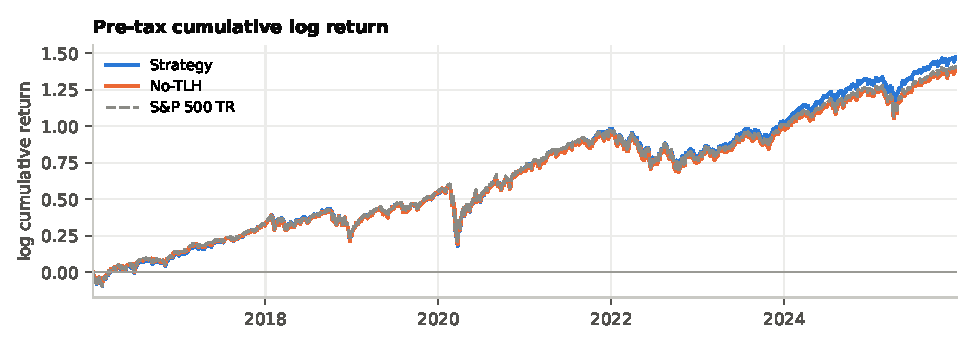
\includegraphics[width=\linewidth]{figures/fig_performance.pdf}
\caption{Pre-tax cumulative log return.}
\label{fig:performance}
\end{figure}

The strategy beat the S\&P 500 TR by 0.75\% a year (Figure~\ref{fig:performance}), but the gap is concentrated in 2024, when the strategy outperformed by 4.8\%. Excluding 2024, the annual gap is 0.34\%. The optimizer forecasts no returns, so this gap reflects active risk rather than a repeatable source of return. Drawdowns were in line with the index. The No-TLH account trailed the index by 0.24\% a year, mainly because about 2\% of its value sat in uninvested cash after whole-share rounding.

\begin{figure}[!h]
\centering
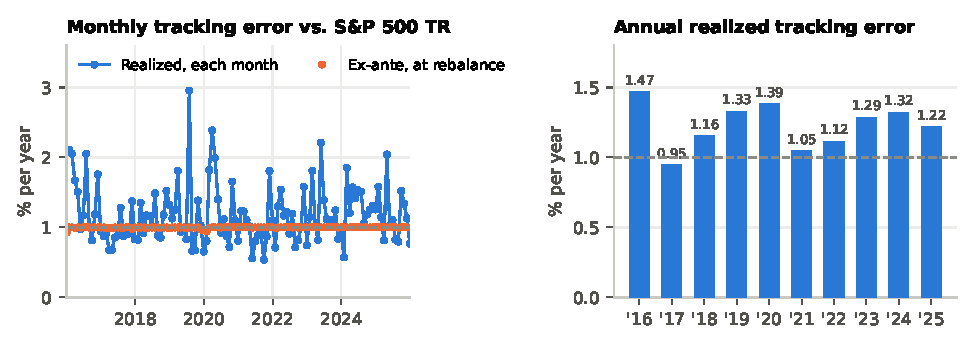
\includegraphics[width=\linewidth]{figures/fig_tracking.pdf}
\caption{Left: realized tracking error within each month (annualized from daily returns) and ex-ante tracking error at each rebalance. Right: realized tracking error by calendar year. Dashed lines mark the 1\% ex-ante limit.}
\label{fig:tracking}
\end{figure}

Ex-ante TE sat at the 1\% limit at almost every rebalance, while realized TE was 1.24\% over the full period. Month by month, realized TE had a median of 1.11\% and exceeded 1\% in 61\% of months (Figure~\ref{fig:tracking}). By calendar year, realized TE ranged from 0.95\% in 2017, the only year below the limit, to 1.47\% in 2016, when heavy harvesting moved the portfolio furthest from the index. The gap reflects drift between monthly rebalances, whole-share rounding and covariance estimation error. Targeting 1\% realized TE would require a tighter ex-ante limit.

\begin{figure}[!h]
\centering
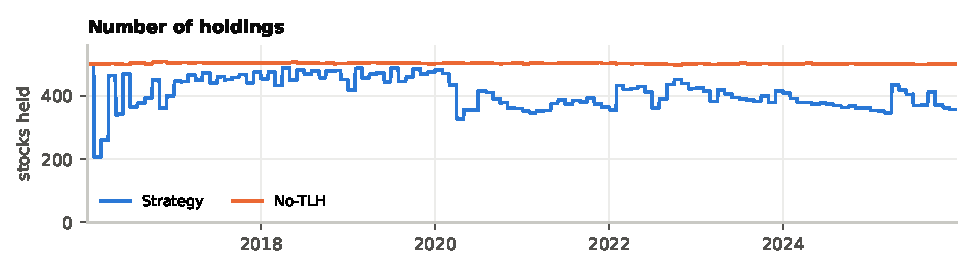
\includegraphics[width=\linewidth]{figures/fig_holdings.pdf}
\caption{Number of stocks held.}
\label{fig:holdings}
\end{figure}

Holdings fell from 502 to 207 in early 2016 as loss positions were sold and only partly replaced, then ranged between 330 and 480, ending at 357 against 501 for No-TLH (Figure~\ref{fig:holdings}). Average annual turnover of 42.3\% (Table~\ref{tab:summary}) is driven up by the first year: in 2016 the new portfolio harvested heavily and one-way turnover reached 183\%. Excluding 2016, turnover averaged 26.7\% a year (Table~\ref{tab:annual}). Of the \$2{,}332 spent on trading in 2016, only \$482 was the initial purchase. Most of the rest came from the February and March rebalances, when the strategy harvested the early-2016 losses.

\begin{table}[!h]
\caption{Annual results. Pre-tax alpha is against the S\&P 500 TR, and tax alpha is against No-TLH, both using calendar-year returns. Turnover is one-way, excluding the initial purchase. Trading cost includes the initial purchase.}
\label{tab:annual}
\small
\begin{tabularx}{\linewidth}{@{}Xrrrrrrrr@{}}
\toprule
\textsf{\textbf{Year}} & \textsf{\textbf{Strategy}} & \textsf{\textbf{S\&P 500 TR}} & \textsf{\textbf{Pre-tax $\alpha$}} & \textsf{\textbf{Tax $\alpha$}} & \textsf{\textbf{Realized TE}} & \textsf{\textbf{Turnover}} & \textsf{\textbf{Trading Cost}} & \textsf{\textbf{Holdings}} \\
\midrule
2016 & 12.1\% & 13.7\% & $-$1.55\% & $+$3.64\% & 1.47\% & 183\% & \$2{,}332 & 400 \\
2017 & 22.8\% & 21.8\% & $+$0.99\% & $+$0.50\% & 0.95\% & 48\% & \$600 & 476 \\
2018 & $-$4.4\% & $-$4.4\% & $-$0.05\% & $+$0.77\% & 1.16\% & 32\% & \$467 & 452 \\
2019 & 30.5\% & 31.5\% & $-$1.00\% & $+$0.85\% & 1.33\% & 30\% & \$454 & 476 \\
2020 & 18.9\% & 18.4\% & $+$0.52\% & $+$1.07\% & 1.39\% & 37\% & \$598 & 361 \\
2021 & 30.0\% & 28.7\% & $+$1.30\% & $-$0.13\% & 1.05\% & 12\% & \$285 & 365 \\
2022 & $-$17.2\% & $-$18.1\% & $+$0.92\% & $+$0.39\% & 1.12\% & 19\% & \$444 & 424 \\
2023 & 27.7\% & 26.3\% & $+$1.40\% & $+$0.55\% & 1.29\% & 29\% & \$734 & 417 \\
2024 & 29.8\% & 25.0\% & $+$4.77\% & $-$0.49\% & 1.32\% & 13\% & \$448 & 363 \\
2025 & 18.4\% & 17.9\% & $+$0.49\% & $+$0.10\% & 1.22\% & 20\% & \$771 & 357 \\
\bottomrule
\end{tabularx}
\end{table}

\subsection{Portfolio Aging}
\label{sec:aging}

Harvesting opportunities shrank as the portfolio aged. Recognized losses equaled 9.1\% of starting NAV in 2016, when every lot had just been bought near cost, and 1.8--3.8\% a year in 2017--2020 (Figure~\ref{fig:aging}). From 2021 they fell to 0.4--1.2\% in most years, with 2023 the exception at 2.8\%. Short-term losses made up 85\% of the \$396{,}000 recognized in total, since lots are most often below cost soon after purchase.

The cost basis fell from 97\% of NAV at inception to 29\% at the end of 2025, while unrealized gains rose to 71\% of NAV (Figure~\ref{fig:basis}). With no external cash flows, new lots come only from reinvested dividends, tax refunds and rebalancing trades, so most of the portfolio sits on gains that rising markets keep widening. Unrealized losses, the stock available to harvest, averaged 1.2\% of NAV in 2016 and only 0.3\% afterwards, rising briefly to 3.4\% in March 2020 and 1.4\% in 2022.

\begin{figure}[!h]
\centering
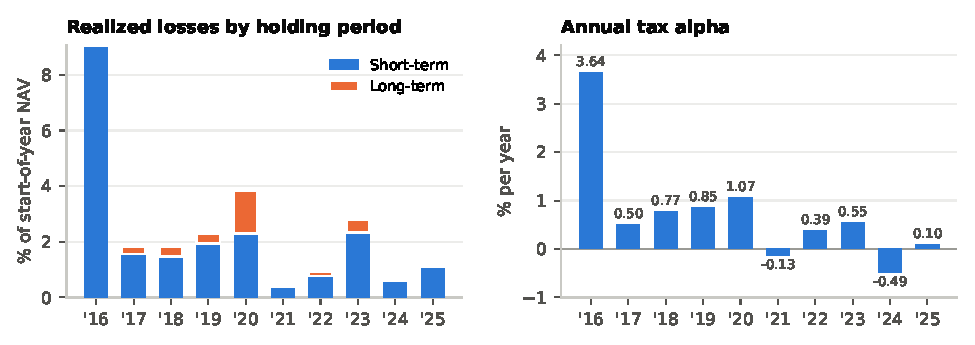
\includegraphics[width=\linewidth]{figures/fig_aging.pdf}
\caption{Left: recognized losses by holding period, as a share of NAV at the start of each year. Right: annual tax alpha against No-TLH.}
\label{fig:aging}
\end{figure}

\begin{figure}[!h]
\centering
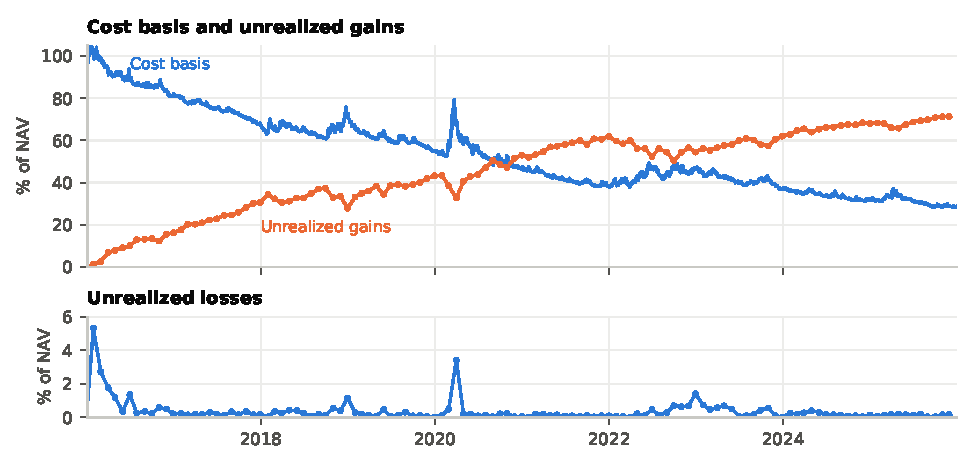
\includegraphics[width=\linewidth]{figures/fig_basis.pdf}
\caption{Top: aggregate cost basis (daily) and unrealized gains summed across lots (at each rebalance), as a share of NAV. Bottom: unrealized losses summed across lots, on their own scale.}
\label{fig:basis}
\end{figure}

Annual tax alpha followed the same path, from 3.64\% in 2016 to an average of 0.40\% in 2017--2025 (Figure~\ref{fig:aging}, right). Market conditions still matter. The 2016 peak partly reflects timing: the portfolio was bought on January 4, the first day of a global sell-off driven by China's stock market crash and oil falling below \$30 a barrel, and the S\&P 500 TR was down 8.9\% by February 11. The COVID-19 crash in March 2020 produced the largest losses after 2016, 3.8\% of NAV. The drawdown was deep enough to push even long-held lots below cost, so long-term losses reached 1.5\% of NAV, 40\% of that year's total and 45\% of all long-term losses over the decade. By contrast, the 2022 bear market produced only 0.9\% of NAV because most lots had appreciated well above cost by then. Strong markets work the other way. In 2021 and 2024 the S\&P 500 TR returned 28.7\% and 25.0\%, yet tax alpha was negative, at $-$0.13\% and $-$0.49\%. Few lots were below cost, so recognized losses fell to 0.4\% and 0.7\% of NAV, while rising prices pushed holdings away from benchmark weights. Trimming them back within the tracking-error limit realized gains, and the strategy paid more tax than No-TLH.

These patterns are consistent with portfolio lock-in. As embedded gains grow, correcting drift from the benchmark increasingly requires realizing gains, which can turn tax alpha negative. The backtest does not isolate this effect from market conditions, so lock-in remains a likely explanation rather than a demonstrated one.

\subsection{The Impact of the Wash-Sale Rule}
\label{sec:wash}
% Source: outputs/wash_metrics_20261122/wash_a (metrics.json, cohorts.json, annual.csv), traced from the final run's ledger.

The wash-sale rule deferred 19\% of harvested losses, but almost all of the deferral was brief. Over the decade the ledger recorded 2{,}593 wash-sale matches, which deferred \$92{,}895 of the \$489{,}252 in gross realized losses (Table~\ref{tab:wash}). Matches fell from 350--540 a year in 2016--2020 to fewer than 110 a year afterwards, in line with the smaller supply of losses in Figure~\ref{fig:aging}.

\begin{table}[!h]
\caption{Wash sales by year of the loss sale. A match pairs a loss sale with one replacement lot bought within 30 days. Gross loss splits into short-term (ST) and long-term (LT) losses. Still deferred is the part of that year's deferred losses not yet released at the end of 2025.}
\label{tab:wash}
\small
\begin{tabular*}{\linewidth}{@{\extracolsep{\fill}}lrrrrrrr@{}}
\toprule
\textsf{\textbf{Year}} & \textsf{\textbf{Matches}} & \textsf{\textbf{Gross Loss}} & \textsf{\textbf{ST Loss}} & \textsf{\textbf{LT Loss}} & \textsf{\textbf{Deferred}} & \textsf{\textbf{Deferred Share}} & \textsf{\textbf{Still Deferred}} \\
\midrule
2016 & 424 & \$118{,}446 & \$118{,}446 & \$0 & \$27{,}893 & 23.5\% & \$1{,}034 \\
2017 & 527 & \$24{,}543 & \$21{,}180 & \$3{,}362 & \$4{,}031 & 16.4\% & \$59 \\
2018 & 496 & \$32{,}294 & \$26{,}595 & \$5{,}699 & \$6{,}412 & 19.9\% & \$87 \\
2019 & 538 & \$36{,}617 & \$30{,}677 & \$5{,}940 & \$5{,}468 & 14.9\% & \$17 \\
2020 & 351 & \$77{,}497 & \$48{,}127 & \$29{,}369 & \$9{,}974 & 12.9\% & \$228 \\
2021 & 30 & \$9{,}418 & \$8{,}684 & \$733 & \$509 & 5.4\% & \$0 \\
2022 & 48 & \$29{,}114 & \$23{,}285 & \$5{,}830 & \$3{,}510 & 12.1\% & \$971 \\
2023 & 104 & \$79{,}824 & \$67{,}293 & \$12{,}531 & \$17{,}011 & 21.3\% & \$617 \\
2024 & 17 & \$26{,}647 & \$23{,}080 & \$3{,}568 & \$6{,}330 & 23.8\% & \$322 \\
2025 & 58 & \$54{,}853 & \$51{,}843 & \$3{,}010 & \$11{,}756 & 21.4\% & \$2{,}137 \\
\midrule
Total & 2{,}593 & \$489{,}252 & \$419{,}210 & \$70{,}042 & \$92{,}895 & 19.0\% & \$5{,}471 \\
\bottomrule
\end{tabular*}
\end{table}

The deferred share stayed between 12\% and 24\% in every year except 2021. By the end of 2025, \$87{,}424 of the \$92{,}895 deferred, or 94\%, had been released, after a median of 60 days, and 84\% were released within the same tax year, leaving that year's tax unchanged. Only \$5{,}471 remained deferred, worth about \$2{,}000 in tax. The largest share comes from 2025, whose replacement lots have had little time to be sold.

The rule therefore costs time value rather than tax savings. It delayed \$36{,}181 of tax benefit in total. Discounting each delayed benefit at 3--8\% a year gives a present-value cost of \$347--\$826 over ten years. Avoiding the rule outright is far more expensive. In a full-sample test that cancelled every wash-triggering order, wash sales disappeared, but after-tax CAGR fell by 1.34\% through cash drag, with cash peaking at 29.7\% of NAV, and drift from the benchmark.

\section{Conclusions}
\label{sec:conclusions}

\subsection{Pros and Cons of Direct Indexing}
\label{sec:proscons}

Direct indexing stays close to the index. Our portfolio tracked the S\&P 500 TR with 1.24\% realized tracking error and drawdowns in line with the index, so it delivers market exposure with little active risk. This makes it suitable for the large pool of risk-averse investors who want index returns rather than active bets.

The strategy also has large capacity. It holds liquid S\&P 500 stocks, trades once a month and does not rely on return forecasts that weaken as assets grow. Its edge comes from each investor's own tax lots, so the same process can run across many separate accounts without crowding.

Owning the stocks directly is what makes harvesting at scale possible. An ETF investor can harvest only when the fund itself trades below cost, which rarely happens after a few years of rising markets. A direct-indexing account holds hundreds of positions and thousands of lots, and individual stocks diverge widely even when the index rises.

The first cost is tracking error. To harvest a loss, the strategy sells a stock and replaces its exposure with other names, which pulls the portfolio away from benchmark weights. Realized tracking error was 1.24\%, against 0.50\% for the No-TLH account that simply replicates SPY, and the average number of holdings fell to 411 from about 503.

The second cost is operational complexity. Every lot must be tracked with its own basis and holding period, every sale checked against purchases within 30 days on either side, and every corporate action applied lot by lot. Execution is harder too. Each rebalance trades hundreds of stocks at once, and liquidity, bid-ask spreads and trading halts differ widely between the largest companies and the smallest index members, so a single order schedule does not fit every name.
\subsection{Value for Investors}
\label{sec:value}

For investors, the value of direct indexing is a lower tax bill on the same market exposure. Over the decade the strategy added 0.75\% a year of tax alpha against an account that holds the same stocks without harvesting. 

Much of this benefit is a deferral rather than a permanent saving. Harvested losses lower the basis of the replacement shares, so the tax deferred today is paid when those shares are eventually sold. A deferral still has value, because the saved tax stays invested and compounds. For an investor who already plans to hold for the long term, harvesting also earns a rate difference. 

The value is therefore highest for a specific investor: one who pays top marginal rates, has outside capital gains to offset each year, holds for a long horizon, and adds new money regularly. New contributions create fresh lots near cost, which slows the aging described in Section~\ref{sec:aging}. For an investor with few outside gains, or one who expects to liquidate soon, much of the benefit is lost.

\subsection{Risks and Limitations}
\label{sec:limitations}

\textbf{Data.} Index weights come from SPY holdings rather than point-in-time S\&P 500 weights. SPY tracks the index closely, but its weights can differ slightly around index changes, and its month-end holdings are assumed known at that day's close. Exits ahead of delistings use dates that were not known in advance, which spares the backtest trading problems a live portfolio would face. Survivorship bias is limited because each month's universe is the historical SPY holding list, including companies later removed or delisted.

\textbf{Tax assumptions.} The largest assumption is that losses offset outside gains in full every year. Without such gains, net losses beyond \$3{,}000 a year would be carried forward, and the tax alpha would be smaller and arrive later. All gains are taxed at top federal rates with no state tax, so investors in other brackets or high-tax states would see different results. Terminal wealth does not deduct tax on unrealized gains. Finally, the simulation uses raw prices and models corporate actions directly, but cash in lieu, rights distributions and similar events are simplified and may be taxed differently in practice.

\textbf{Backtest.} Results come from a single ten-year path, and the start date matters. The portfolio was bought just before the early-2016 sell-off, which produced the largest tax alpha of any year. Trades fill at the closing price with a flat 5 bp cost. The backtest ignores slippage, the bid-ask spread and market impact, which would raise the cost of heavy trading.

\textbf{Strategy.} The optimizer is myopic. It solves each monthly rebalance on its own and ignores how today's trades change future harvesting opportunities and future tax. Selling a loss today, for example, lowers the basis of the replacement shares and raises the tax on their later sale. The result is therefore not optimal over the whole horizon, and within each rebalance Step~1 is a local search with no global-optimality guarantee. The risk model is also imperfect: realized tracking error ran above the ex-ante limit in nine of ten years, and active risk moved pre-tax returns by as much as 4.8\% in a single year.

\textbf{Portfolio aging and wash sales.} Tax alpha fell as embedded gains grew after a few years, and the backtest cannot separate aging from market conditions. The wash-sale rule deferred 19\% of harvested losses. Most were released within months, but the Step~1 penalty only discourages trades that trigger the rule and does not prevent them.

\section{Next Steps}
\label{sec:next}

\textbf{A more exact, convex formulation.} A more accurate convex objective might let the optimizer solve the problem directly instead of searching for directions. For example, with purchases and lot sales as separate variables the costs become linear, and the remaining no-buy-and-sell rule can be handled with one binary variable per loss stock. The result is a mixed-integer SOCP that a commercial solver may solve to global optimality.

\textbf{Multi-period optimization.} The current optimizer looks only at the next rebalance. Optimizing several future rebalances on simulated return paths, or training a reinforcement-learning agent, might help weigh a harvest today against the higher tax on lower-basis replacement shares later.

\textbf{Wash-sale-aware constraints.} Another direction is to search for better solutions that do not trigger wash sales at all. Step~2 might forbid the trade direction that would trigger the rule, which keeps it convex, while a highly correlated substitute holds the exposure until the window closes.

\textbf{Harvesting frequency.} Monthly rebalancing misses losses that appear and recover within the month. A daily or weekly loss scan between rebalances is a simple way to test how much of this short-lived opportunity can be captured.

\textbf{Gain realization against aging.} Realizing some long-term gains on purpose may slow portfolio aging. One option is to sell the most appreciated lots up to the amount of losses harvested in the same year, resetting the cost basis at little tax cost.

\textbf{Tighter control of tracking error.} Realized tracking error ran above the ex-ante limit. A convex penalty on the size of position changes, combined with a slightly lower ex-ante limit, may bring it closer to 1\%.

\textbf{Cash flows.} Regular contributions add new lots near cost. Simulating them, along with withdrawals, may show how far new money can slow the decline in tax alpha.

\textbf{Calibration of $\gamma$.} The choice of $\gamma=0.5$ deserves an empirical check. Rerunning the backtest over a grid of $\gamma$ between 0.25 and 1 and several tracking-error limits might map the trade-off between tax alpha and tracking error.

\section*{Use of AI Tools}
\label{sec:ai}

I used AI assistants (ChatGPT and Claude) as research and engineering aids throughout the project. They helped me collect academic papers and industry reports, review my code, set up example test cases, and reorganize the code to make it shorter and easier to read. I also used them to test my ideas and to look for bugs and limitations I had not considered. Finally, they drafted parts of the \LaTeX{} source and helped me adjust the layout. I checked all design choices and reported results against my code and its outputs.


\end{document}
